% Default Inputs
% Seiten-Layout
\documentclass[a4paper,12pt]{scrartcl}	%Seitenlayout allgemein
%\documentclass[a4paper,12pt]{article}		%Seitenlayout allgemein
\usepackage[left=3cm, right=2.5cm, top=2.5cm, bottom=2.5cm, footskip=0.7cm]{geometry}						%Seitenränder
\usepackage{fancyhdr}				%Kopf- und Fußzeilen-Manipulation
\pagestyle{empty}					%Seitenzahl, empty=ohne, 
\fancyhf{} 							%alle Kopf- und Fußzeilenfelder bereinigen
\usepackage{lscape}					%Querformat in Bereich
%\usepackage[section]{placeins}


% Text-Layout
\usepackage[ngerman]{babel} %deutsche Sprache+Umlaute
\usepackage[latin1, utf8]{inputenc}
\usepackage[T1]{fontenc} %Codieung7-auf8-Bit
\usepackage{marvosym} %Symbole
\DeclareUnicodeCharacter{20AC}{\EUR} %z.B.Euro-Symbol
\usepackage{nameref} %für-Überschriften
\addto\captionsngerman{\renewcommand{\refname}{Literaturverzeichnis}}
\usepackage{lmodern}				%Vektorisierte Schrift
\usepackage[scaled]{uarial}			%Arial
\usepackage[onehalfspacing]{setspace}	%1,5-facher Zeilenabstand



% Überschriften



% Forms-Formatierung
\usepackage{parskip}				%Absätze
\usepackage{array}					%Tabellen
\usepackage[format=hang,font={footnotesize,sc}, 
labelfont={bf},margin=1cm,aboveskip=5pt,
position=top]{caption} 				%Tabellenunterschriften, evtl. Formatieren
\usepackage{pifont}					%Dingbats-Symbole (siehe Tabelle)
\usepackage{enumerate}				%Aufzählungen: a A i I 1
\usepackage{graphicx}				%Bilder



% Verzeichnisse
\usepackage{titletoc}				% Inhaltsverzeichnis umdefinieren
\usepackage{tocloft}					% Abbildungsverzeichnis umdefinieren
\usepackage{acronym}				%Abkürzungsverzeichnis



% Codes
\usepackage[dvipsnames]{xcolor}	% Color
\usepackage{listings}				%Weiteres Verzeichnis
\lstset{captionpos=b}				% Caption after Code



% Anhang
\usepackage[toc,page]{appendix}
\renewcommand{\appendixtocname}{Anhang}
\renewcommand{\appendixpagename}{Anhang}






% Drawings
\usepackage{tikz}				%Graphik-Elemente / Zeichnen



% Programming Functions
\usepackage{amsmath}
\usepackage{amssymb}
\usepackage{empheq}
\usepackage{mathrsfs}
\usepackage{theorem}
\usepackage{xifthen}




% Layout Überschriften im TOC
\newcommand{\TocLayoutE}[3]{\titlecontents{#1}[#2em]{}{\contentslabel{0em}}{\vspace*{#3cm}}{\titlerule*[0.3pc]{.}\contentspage}}
\newcommand{\TocLayoutD}[4]{\titlecontents{#1}[#2em]{}{\contentslabel{#4em}}{\vspace*{#3cm}}{\titlerule*[0.3pc]{.}\contentspage}}
\newcommand{\TocLayoutA}[4]{\titlecontents{#1}[#2em]{}{\contentslabel{#4em}}{\vspace*{#3cm}}{\titlerule*[0.3pc]{}}}

\newcommand{\TocStdSectionE}{\TocLayoutE{section}{0}{0}}
\newcommand{\TocStdSectionD}{\TocLayoutD{section}{1.5}{0}{1.5}}
\newcommand{\TocStdSectionA}{\TocLayoutA{section}{0}{0}{1.5}}

\newcommand{\TocStdSubSectionE}{\TocLayoutE{subsection}{3}{0.25}}
\newcommand{\TocStdSubSectionD}{\TocLayoutD{subsection}{3}{0.25}{2.25}}
\newcommand{\TocStdSubSectionA}{\TocLayoutA{subsection}{3}{0.25}{2.25}}

\newcommand{\TocStdSubSubSectionE}{\TocLayoutE{subsubsection}{4.5}{0.25}}
\newcommand{\TocStdSubSubSectionD}{\TocLayoutD{subsubsection}{4.5}{0.25}{3}}
\newcommand{\TocStdSubSubSectionA}{\TocLayoutA{subsubsection}{4.5}{0.25}{3}}



\usepackage{chngcntr}

% Layout PaygeStyle
\newcommand{\PagestyleStdPre}{\pagestyle{empty}}
\newcommand{\PagestyleStdFormal}{\pagestyle{fancy} \setcounter{page}{1} \pagenumbering{Roman} \fancyhf[fr]{\thepage} \TocStdSectionE \TocStdSubSectionE \TocStdSubSubSectionE \captionsetup[figure]{list=no}}
\newcommand{\PagestyleStdContent}{\pagestyle{fancy} \setcounter{page}{1} \pagenumbering{arabic} \fancyhf[fr]{\thepage} \TocStdSectionD \TocStdSubSectionD \TocStdSubSubSectionD \captionsetup[figure]{list=yes}}
\newcommand{\PagestyleStdSuf}{\pagestyle{empty} \TocStdSectionA \TocStdSubSectionA \TocStdSubSubSectionA \captionsetup[figure]{list=no}}
\newcommand{\PagestyleStdAppendix}{\pagestyle{fancy} \setcounter{page}{1} \pagenumbering{roman} \renewcommand{\thepage}{\thesection-\arabic{page+1}} \counterwithin{page}{section} \TocLayoutA{section}{1.5}{0}{1.5}}

\renewcommand{\headrulewidth}{0pt}
\renewcommand{\footrulewidth}{0pt}



% Layout Codes
\lstdefinestyle{Style_Java}{
	language=Java,
	basicstyle=\tiny,
	backgroundcolor=\color[rgb]{.93,.93,.93},
	commentstyle=\color[rgb]{.17,.55,.17},
	keywordstyle=\color[rgb]{1,.08,.58},
	numberstyle=\tiny\color[rgb]{.1,.2,.3},
	stringstyle=\color[rgb]{0,0,.53},
	numbers=left,
	stepnumber=1,
	breakatwhitespace=true,
	breaklines=true,
	showspaces=false,
	showstringspaces=false,
	showtabs=false,
	tabsize=2
}

\lstdefinestyle{Style_CPP}{
	language=C++,
	basicstyle=\tiny,
	backgroundcolor=\color[rgb]{.93,.93,.93},
	commentstyle=\color[rgb]{.17,.55,.17},
	keywordstyle=\color[rgb]{0.7,.05,.5},
	numberstyle=\tiny\color[rgb]{.1,.2,.3},
	stringstyle=\color[rgb]{0,0,.53},
	numbers=left,
	stepnumber=1,
	breakatwhitespace=true,
	breaklines=true,
	showspaces=false,
	showstringspaces=false,
	showtabs=false,
	tabsize=2
}

\lstdefinestyle{Style_IOC}{
	language=XML,
	basicstyle=\tiny,
	backgroundcolor=\color[rgb]{.93,.93,.93},
	commentstyle=\color[rgb]{.25,.25,.25},
	keywordstyle=\color[rgb]{0,0,0},
	numberstyle=\tiny\color[rgb]{0,0,0},
	stringstyle=\color[rgb]{0,0,0},
	numbers=left,
	stepnumber=1,
	breakatwhitespace=true,
	breaklines=true,
	showspaces=false,
	showstringspaces=false,
	showtabs=false,
	tabsize=2
}

\newcommand{\CodePkg}[1]{\texttt{\textit{\textcolor{RedViolet}{#1}}}}
\newcommand{\CodeClass}[1]{\texttt{\textcolor{BlueGreen}{#1}}}
\newcommand{\CodeMeth}[1]{\texttt{#1}}
\newcommand{\CodeVar}[1]{\texttt{#1}}











\usepackage{amsmath}
\usepackage{amssymb}
\usepackage{empheq}
\usepackage{mathrsfs}
\usepackage{theorem}
%Private Commands
\newcommand{\idR}{in der Regel}
\newcommand{\zB}{zum Beispiel}
\newcommand{\bspw}{beispielsweise}
\newcommand{\bzw}{beziehungsweise}
\newcommand{\sg}[1][]{so genannte#1}
\newcommand{\ggfShort}{ggf.}
\newcommand{\ggf}{gegebenenfalls}
\newcommand{\ua}{unter anderem}
\newcommand{\uU}{unter Umständen}
\newcommand{\evtl}{eventuell}

\newcommand{\Anmerkung}[1]{\begin{footnotesize}\textit{Anmerkung:} #1\end{footnotesize}}
\newcommand{\note}[1]{\Anmerkung{#1}}
\newcommand{\vgl}[1]{(vgl. \cite{#1})}
\newcommand{\comp}[1]{\mbox{(vgl. \cite{#1})}}
\newcommand{\compB}[2]{\mbox{(vgl. \cite{#1}} und \cite{#2})}
\newcommand{\compC}[3]{\mbox{(vgl. \cite{#1},} \cite{#2} und \cite{#3})}

\newcommand{\refFul}[1]{\ref{#1} \mbox{(Seite \pageref{#1})}}
\newcommand{\refCap}[1]{\mbox{Kapitel \ref{sec:#1}} \textit{\nameref{sec:#1}} \mbox{(Seite \pageref{sec:#1})}}
\newcommand{\refCapShort}[1]{\ref{sec:#1} \textit{\nameref{sec:#1}} \mbox{(Seite \pageref{sec:#1})}}
\newcommand{\refApp}[1]{\mbox{Anhang \ref{sec:#1}} \textit{\nameref{sec:#1}}}
\newcommand{\refAbb}[1]{\refImg{#1}}
\newcommand{\refImg}[1]{\refImgShort{#1} \mbox{(Seite \pageref{#1})}}
\newcommand{\refImgShort}[1]{\mbox{Abbildung \ref{#1}}}
\newcommand{\refTab}[1]{\mbox{Tabelle \ref{#1}} \mbox{(Seite \pageref{#1})}}
\newcommand{\missing}[1][]{\textcolor{red}{BESCHREIBUNG! \begin{footnotesize}\textit{#1}\end{footnotesize}}}




\newcommand{\TOCLF}{\addtocontents{toc}{\protect\clearpage}}

% Specific Inputs
%Private Commands
\newcommand{\Wartung}[1][]{Server-Wartung#1}
\newcommand{\Server}[1][]{Service-Server#1}
\newcommand{\RevEng}[1][]{\textit{Reverse Engineering#1}}
\newcommand{\RevEngN}[1][]{Reverse Engineering#1}
\newcommand{\Doku}{Software Dokumentation}
\newcommand{\UserDoku}{\textit{Benutzerdokumentation}}
\newcommand{\Entwicklung}{Software-Entwicklung}
\newcommand{\Entwickler}{Software-Entwickler}
\newcommand{\ERD}{\textit{Entity Relationship Diagramm}}
\newcommand{\CLI}{\textit{Command Line Interface}}
\newcommand{\SSH}{\textit{Secure Shell}}



\newcommand{\www}{\textit{world wide web}}
\newcommand{\UC}[1][]{Use-Case#1}
\newcommand{\UCD}[1][]{\UC -Diagramm#1}
\newcommand{\FC}[1][]{Function-Call#1}
\newcommand{\FCD}[1][]{\FC -Diagramm#1}
\newcommand{\VM}[1][]{\textit{virtuelle#1 Maschine}}
\newcommand{\OS}[1][]{Betriebssystem#1}
\newcommand{\Auth}[1][]{Authentifizierung#1}




\newcommand{\Config}[1][]{Konfigu\-ration}
\newcommand{\ConfigF}[1][]{\Config[s]datei}


\newcommand{\MCU}[1][]{Micro\-controller#1}
\newcommand{\uProc}[1][]{Mikro\-prozessor#1}
\newcommand{\STM}{\textit{STMicroelectronics}}
\newcommand{\STMDZ}{\textit{STM32}}
\newcommand{\MCUDZ}[1][]{\STMDZ-\MCU[#1]}

\newcommand{\POC}{\textit{Proof of Concept}}

\newcommand{\cpp}{\textit{C++}}


\newcommand{\EmbSys}{\textit{Embedded Systems}}




\newcommand{\Stack}{\textit{automatic storage duration}-Bereich}
\newcommand{\Heap}{\textit{dynamic storage duration}-Bereich}
\newcommand{\Static}{\textit{static storage duration}-Bereich}
\newcommand{\STL}{\textit{Standard Template Library}}



\newcommand{\ROS}{\textit{ROS}}
\newcommand{\Quad}[1][]{Quadrokopter#1}
\newcommand{\COEX}{\textit{COEX}}
\newcommand{\Clover}{\textit{Clover 4.20}}

\newcommand{\clean}{\textit{Clean Archirecture}}
\newcommand{\VO}{\textit{Value-Object}}













% Autor-Informationen
\newcommand{\AutorTitel}{B.Ing.}
\newcommand{\AutorVorname}{Michael}
\newcommand{\AutorNachname}{Maag}
\newcommand{\AutorAnschrift}{Freidorfstraße 14}
\newcommand{\AutorPLZ}{97957}
\newcommand{\AutorStadt}{Wittighausen}
\newcommand{\AutorMatrNr}{6170558}
\newcommand{\AutorAngestrebterAbschluss}{Bachelor of Science}
\newcommand{\AutorStudiengang}{Informatik}
\newcommand{\AutorKurs}{TINF19B1}

% DHBW-Informationen
\newcommand{\DHBW}{DHBW Karlsruhe}
\newcommand{\DHBWAnschrift}{Erzbergerstraße 121}
\newcommand{\DHBWPLZ}{76133}
\newcommand{\DHBWStadt}{Karlsruhe}
\newcommand{\DHBWLogo}[1][1.5]{\includegraphics[keepaspectratio=true, height=#1cm]{DefaultContent/200803_DefaultDHBW_Logo \DHBWStadt}}

% Ausarbeitung-Informationen
\newcommand{\AusarbeitungThema}{Initialsensorenbasierte Positionsregelung eines Indoor-Quadrokopters}
\newcommand{\AusarbeitungBezeichnung}{T3100}
\newcommand{\AusarbeitungZeitraum}{6 Monate}
\newcommand{\AusarbeitungAbgabeDatum}{16.05.2022} % Check again!
\newcommand{\BetreuerFirma}{}
\newcommand{\BetreuerDHBW}{Prof. Dr. Marcus Strand}



% Weitere Funktionen
\newcommand{\Unterschrift}{\vspace{1cm}\begin{tabbing}
\hspace{10cm}\= \kill
\underline{\hspace{5cm}} \> \underline{\hspace{5cm}}\\
\AutorStadt, \AusarbeitungAbgabeDatum \> Unterschrift
\end{tabbing}}




\newcommand{\Arbeit}{Projektarbeit}

% Default Inputs with 'Info - Autor' Data
% Setup PDF
\usepackage{hyperref}
\hypersetup{
  pdftitle    = {},
  pdfsubject  = {},
  pdfauthor   = {},
  pdfkeywords = {} ,
  pdfcreator  = {},
  pdfproducer = {LaTeX with hyperref}
}							%PDF-Einstellungen












\begin{document}
%Private Commands which have to be within \begin{Document}
\newcommand{\comSec}[2][]{\section{#2} \ifthenelse{\isempty{#1}}{\label{sec:#2}}{\label{sec:#1}}}
\newcommand{\comSSec}[2][]{\subsection{#2} \ifthenelse{\isempty{#1}}{\label{sec:#2}}{\label{sec:#1}}}
\newcommand{\comSSSec}[2][]{\subsubsection{#2} \ifthenelse{\isempty{#1}}{\label{sec:#2}}{\label{sec:#1}}}
\newcommand{\comPar}[2][]{\textbf{#2} \ifthenelse{\isempty{#1}}{\label{sec:#2}}{\label{sec:#1}}}
\newcommand{\comSPar}[2][]{\textit{\textbf{#2}} \ifthenelse{\isempty{#1}}{\label{sec:#2}}{\label{sec:#1}}}

\newcommand{\newSec}[3][]{%
	\ifthenelse{\equal{#3}{1}}{\comSec[#1]{#2}}{}
	\ifthenelse{\equal{#3}{2}}{\comSSec[#1]{#2}}{}
	\ifthenelse{\equal{#3}{3}}{\comSSSec[#1]{#2}}{}
	\ifthenelse{\equal{#3}{4}}{\comPar[#1]{#2}}{}
	\ifthenelse{\equal{#3}{5}}{\comSPar[#1]{#2}}{}
	
	\ifthenelse{\equal{#3}{-1}}{\comSec[#1]{#2} \setcounter{page}{1}}{} % Appendix Sections
}





\newcommand{\Cellln}[1]
{
	\begin{tabular}[c]{@{}l@{}}#1\end{tabular}
}


%Private Commands

















%Private Commands
\newcommand{\ROS}{\textit{ROS}}
\newcommand{\Node}[1][]{\textit{ROS-Node#1}}
\newcommand{\Topic}[1][]{\textit{ROS-Topic#1}}
\newcommand{\Service}[1][]{\textit{ROS-Service#1}}

\newcommand{\rTopic}[1]{\Topic \texttt{\textcolor{magenta}{#1}}}












\PagestyleStdPre

% Default Content
\thispagestyle{empty}


\DHBWLogo
\vspace{2cm}


\begin{center}
\LARGE{\textbf{\AusarbeitungThema}}
\vspace{0.25cm}

\Large{\textbf{\AusarbeitungBezeichnung}}
\vspace{0.25cm}

für die Prüfung zum \\
\AutorAngestrebterAbschluss
\vspace{0.25cm}

im Studiengang \AutorStudiengang \\
an der \DHBW
\vspace{0.25cm}

von\\
\textbf{\AutorVorname\ \AutorNachname} \\
\AusarbeitungAbgabeDatum

\end{center}
\vspace{0.5cm}


\begin{tabbing}
\hspace{8cm} \= \kill
Bearbeitungszeitraum \> \AusarbeitungZeitraum\\
Matrikelnummer \> \AutorMatrNr\\
Gutachter der \DHBW \> \BetreuerDHBW
\end{tabbing}

\clearpage
%\thispagestyle{empty}


\begin{center}
\huge{\textbf{Sperrvermerk}}
\par
\vspace{2cm}
\end{center}

Der Inhalt dieser Arbeit darf weder als Ganzes noch in Auszügen Personen außerhalb des Prüfungsprozesses und des Evaluationsverfahrens zugänglich gemacht werden, sofern keine anderslautende Genehmigung vom Dualen Partner vorliegt.

\Unterschrift
\clearpage

\thispagestyle{empty}
\pagenumbering{gobble}


\AutorVorname\ \AutorNachname\\
\AutorAnschrift\\
\AutorPLZ\ \AutorStadt\
\vspace{2cm}



\begin{center}
\huge{\textbf{Eigenständigkeitserklärung}}
\vspace{2cm}
\end{center}

Ich versichere hiermit, dass ich meine Ausarbeitung \AusarbeitungBezeichnung\ mit dem Thema \grqq \AusarbeitungThema \grqq\ selbstständig verfasst und keine anderen als die angegebenen Quellen und Hilfsmittel benutzt habe.
Ich versichere zudem, dass die eingereichte elektronische Fassung mit der gedruckten Fassung übereinstimmt.

\Unterschrift

\thispagestyle{empty}

\clearpage

% Indecies
\setcounter{tocdepth}{3}

\tableofcontents
%\begin{minipage}[][1cm][1cm]{1cm}
%\thispagestyle{empty}
%\end{minipage}

\thispagestyle{empty}
\clearpage





\clearpage
\PagestyleStdFormal

\listoffigures
\addtocontents{lof}{\protect\thispagestyle{fancy}}
\addcontentsline{toc}{section}{Abbildungsverzeichnis}

\clearpage

\input{211008_MM_T3100_Verzeichnisse - Abkürzungen.tex}
\listoftables
\addcontentsline{toc}{section}{Tabellenverzeichnis}

\clearpage

\clearpage
\listofequs
\clearpage
\addcontentsline{toc}{section}{Code-Verzeichnis}
\renewcommand{\lstlistingname}{Code}
\renewcommand*{\lstlistlistingname}{Code-Verzeichnis}	%Change Name of List
\lstlistoflistings         % Liste der Listings


\clearpage

% BEISPIEL



%\begin{lstlisting}[caption=[short Caption for List]{long Caption}, label={}, captionpos=b]
%CODE
%\end{lstlisting}

%\lstinputlisting[language=make,         % Welche Sprache, see listings-Dokumentation
%                 style=algoBericht,     % Benutze oben definierten Stil
%                 label={algo-makefile}, % Label für \ref{..}
%                 basicstyle=\tiny\sffamily,
%                 captionpos=b,
%		 caption={Das Makefile}]{Makefile.} % Überschrift, Dateiname der zu inkludieren Datei

% ACHTUNG: ProTeXT / Windows hat hier ein Bug: "Makefile" ohne Punkt am Ende wird nicht gefunden.
%          ($%&/ DOS-Legacy :-(
%          Daher muss für Linux eine Datei "Makefile." (mit Punkt am Ende) als Symlink auf "Makefile"
%          angelegt werden und hier "Makefile." angegeben werden. Das ist nur notwendig,
%          wenn der Dateiname keinen Suffix hat....



% Specific Content
\clearpage
\PagestyleStdContent


\newSec{Einleitung}{1}


\vspace{1cm}
\begin{center}
\textbf{\grqq Über den Wolken muss die Freiheit wohl grenzenlos sein.\grqq}\\
\vspace{0.5cm}
aus dem Lied \textit{Über den Wolken} von Reinhard Mey, 1973 \cite{Einl1}
\end{center}
\vspace{1cm}


Schon lange sehnten sich Menschen danach, fliegen zu können. Eine der bekanntesten Geschichten ist die Mythologie über Ikarus, der auf der Flucht aus dem Labyrinth auf der Insel Kreta mit selbstgebauten Flügeln der Sonne zu nahe kam und daraufhin ins Meer stürzte. \comp{Einl2}\\
Leonardo da Vinci deutete Ende des 15. Jahrhunderts in den \textit{Pariser Manuskripten} die Funktionsweise eines Helikopters \bzw\ einer Luftschraube an. \comp{Einl3}

Diverse Paket-Lieferdienste planen, \Quad\ in Ballungsgebieten zum Versand von Paketen einzusetzen. \comp{Einl4}

Zur Wegplanung ist eine korrekt berechnete Pose (Position und Orientierung) des \Quad[s] notwendig. Hierzu können diverse Sensoren eingesetzt werden, welche an den Fuggeräten eingesetzt werden.\\
In dieser \Arbeit\ wurden Initialsensoren als mögliche Herangehensweise ausgewählt. Als Grundlage für die Auswahl kann die einfache Aufarbeitung der Daten genannt werden. Zudem wurden bereits erfolgreich Projekte mit diesem Konzept umgesetzt. \compB{Paper3}{Paper4}






\vspace{5cm}
\note{Für diese Ausarbeitung werden fachliche Begrifflichkeiten vorausgesetzt, sofern diese nicht innerhalb der Ausarbeitung erklärt werden. Sind Begriffe für Lesende unklar, sind diese an geeigneter Stelle nachzuschlagen. Auf eine voranstehende Erklärung aller genutzten und nicht näher erklärten Begriffe wird in dieser Ausarbeitung verzichtet, um den Rahmen dieser Arbeit einhalten zu können.}







						% Section
\clearpage
\newSec{Problemstellung}{1}

Fluggeräte jeder Ausführung können durch Umwelteinflüsse von ihrer Position abgetrieben werden \vgl{Ballon}. Während der Versuchsdurchführung von Studierenden der \DHBW\ an einem \Quad\ hat sich gezeigt, dass sich das Halten einer Position für Piloten mit geringer Erfahrung als schwierig erweist. Beschädigungen der in Laborversuchen eingesetzten Hardware ist zu vermeiden.
Die Versuchsdurchführung \textit{Höhenregelung}\footnote{Bei dem Laborversuch \textit{Höhenregelung} sollen Studierende eine ROS-Node erstellen, welche eine konstante Flughöhe des \Quad[s] ermöglicht. Hierzu wird als Rückführungsgröße des Regelkreises die Abstandsmessung zwischen \Quad\ und der daruterliegenden Ebene eingesetzt.} soll für die Studierenden dahingehend vereinfacht werden, alsdass der eingesetzte \Quad\ die horizontale Bewegung selbstständig regelt.

Zu entwickeln ist eine Positionsregelung auf Basis der verfügbaren Beschleunigungswerte der Drohne. Optional kann die Regelung um ein bildgestütztes System erweitert werden.

Für die Positionsregelung können unterschiedliche Modi entwickelt werden:
\begin{itemize}
\item Halten der Position nach einer manuellen Positionsänderung
\item Anfliegen von vorgegebenen Positionen. Hierbei ist ein Überschwingen möglichst zu vermeiden.
\end{itemize}

Durch die Anschaffung eines neuen \Quad[s] erweitert sich die Aufgabenstellung um den Aufbau des Bausatzes und die Inbetriebnahme des \Quad[s], an dem die Positionsregelung implementiert werden soll.
Die Anpassung der Versuchsbeschreibung an die geänderte Hardware ist gewünscht.

Eine tabellarisch angelegtes Lastenheft ist \missing[im Kapitel Anhang...] einzusehen.






					% Section
\clearpage






\clearpage
\newSec{Methodik}{1}



						% Section
\newSec[SW]{Eingesetzte Software}{2}

In diesem Kapitel sollen die für diese \Arbeit\ eingesetzten Softwares genannt, um eine Reproduktion der Ergebnisse gewährleisten zu können.


\note{Die Ausführungen der eingesetzten Software beziehen sich auf den Umgang mit der Drohne \textit{ArDrone 2.0}. Für die Interaktion mit der Drohne \textit{Clover 4.20}, weche zum Projektbeginn eingesetzt wurde, wurde aktuellere Software eingesetzt.}


\newSec{ROS}{3}
Das \textit{Robot Operating System} (\ROS) ist eine \textit{Open Source} Bibliothek, welche dem Nutzer eine modulare Architektur ermögicht.
Hierbei kommunizieren \textit{Nodes} mittels \textit{Messages} miteinander.\vgl{ros1}

Die \ROS\ Versionen werden jeweils mit Namen versehen, wobei die Anfangsbuchstaben der Versionen der alphabetischen Nummerierung entsprechen. In diesem Projekt wurde die \ROS-Version \textit{Indigo} eingesetzt.
Diese Version wird auf Grund der Anforderungen des \textit{Driver}-Package \textit{ardrone\_autonomy} eingesetzt. Der Einsatz der aktuellsten \ROS-Version \textit{noetic} in Zusammenspiel mit \textit{Ubuntu 20.04} konnte das gewünschte Ergebnis nicht erzielen.

Die \ROS\textit{-Nodes} wurden mittels \textit{catkin} compiliert.
Für eine korrekte Kompilierung müssen \textit{CMakeList.txt}-Dateien den Befehl \texttt{add\_compile\_options(-std=c++11)} beinhalten.


\newSec{Ubuntu - Betriebssystem}{3}
Als Betiebtssystem wird das \textit{UNIX}-basierte Betriebssystem \textit{Ubuntu} auf einer \VM\ in der Version 14.04 eingesetzt.
Die Auswahl dieser Version gründet auf den Anforderungen der \ROS \textit{Indigo}-Version.\comp{rosVersion}

Die \VM\ wird durch die Software \textit{VMWare Workstation 15 Pro} visualisiert.


\newSec{Visual Studio - IDE}{3}
\missing\









					% SubSection


\clearpage
\newSec[Quads]{\Quad\ als System}{1}







\newSec{Geometrien}{2}
Die Rotoren von Drohnen können in zwei verschiedenen Anordnungen angebracht werden. in diesem Kapitel sollen diese Anordnung näher beschrieben werden.





\newSec[Plus]{\textbf{+}-Anordnung}{3}




\missing[für roll und pitch wird die Drehzahl die Rotoren auf der jeweiligen Achse entgegengesetzt manipuliert.]
\missing[für eine Drehung um die z-Achse werden die Rotoren der x- und y-Achse entgegengesetzt manipuliert.]



\newSec[X]{\textbf{x}-Anordnung}{3}
\missing\




\newSec{Freiheitsgrade}{2}




6 Freiheitsgrade, tatsächlich 4 individuell regelbar.

\missing[Bild der Kräfte an der Drohne, wenn diese aus der horizontalen Ebene geneigt ist.]





					% Section






\clearpage
\newSec{Regelsysteme}{1}



Evtl Norm „IEC 60050-351 Internationales Elektrotechnisches Wörterbuch – Teil 351: Leittechnik“ zitieren, auf jeden Fall als Grundlage heranziehen.
+ Vorlesung Regelungstechnik von Studium MB13VT





\newSec[Regelerarten]{Arten von Reglern}{2}



\newSec[ControlP]{P-Regler}{3}



\newSec[ControlI]{I-Regler}{3}



\newSec[ControlD]{D-Regler}{3}



\newSec[ControlPID]{PID-Regler}{3}



\newSec[ControlPT]{PT-Regler}{3}








					% Section
\newSec{Regelkreis}{2}

Im Allgemeinen grenzen sich die Konzepte \textit{steuern} und \textit{regeln} durch die Eigenschaft der Rückkopplung des Systems ab. Gesteuerte Systeme wirken lediglich auf Aktoren, wobei geregelte Systeme die Abweichung des \textit{Ist}-Zustandes vom \textit{Soll}-Zustand ermitteln und eine geeignete Veränderung erzielen sollen.\comp{IEC60050-351}




\begin{figure}[ht!]
\vspace{0.25cm}
\begin{center}
\fbox{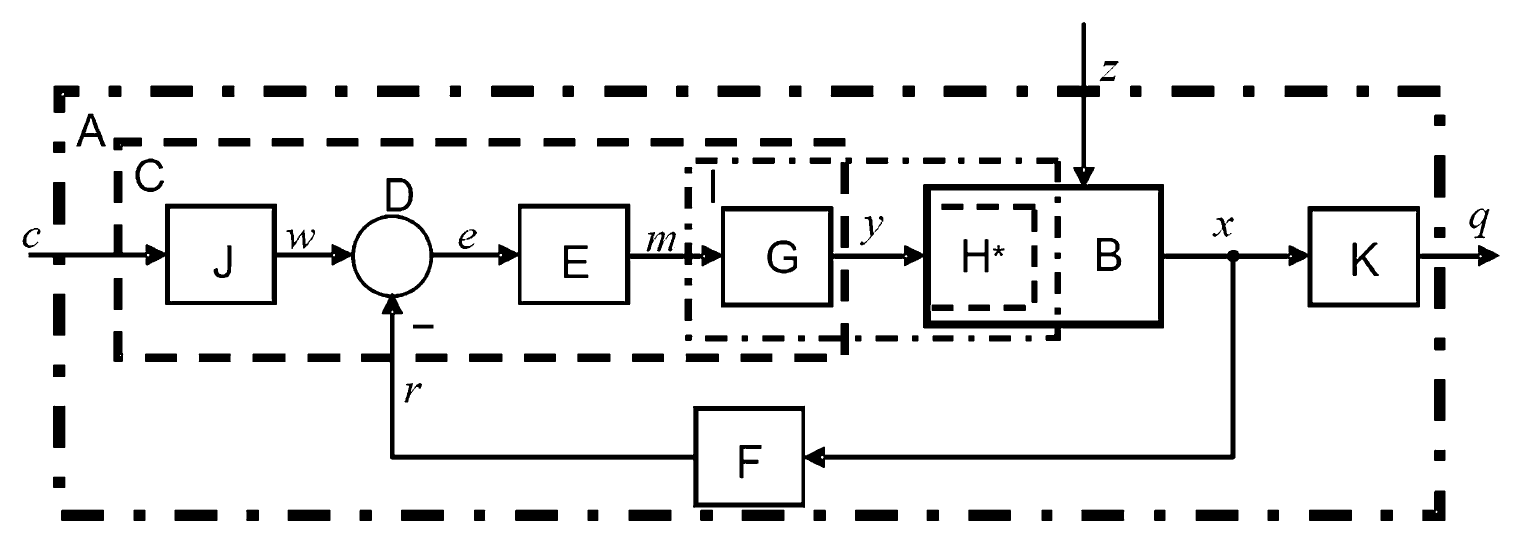
\includegraphics[width=15cm]{Pictures/Control Schema.png}}

\begin{tabular}{ll|ll}
	A  & Regelungssystem       & K & Bildung der Aufgabengröße \\
	B  & Regelstrecke          & c & Zielgröße                 \\
	C  & Regeleinrichtung      & w & Führungsgröße             \\
	D  & Vergleichsglied       & e & Regeldifferenz            \\
	E  & Regelglied            & m & Reglerausgangsgröße       \\
	F  & Messglied             & y & Stellgröße                \\
	G  & Steller               & z & Störgröße                 \\
	H* & Stellglied            & x & Regelgröße                \\
	I  & Stelleinrichtung      & q & Aufgabengröße             \\
	J  & Führungsgrößenbildner & r & Rückführgröße            
\end{tabular}
\caption{Allgeimeines Schema eines Regelkreises \cite{IEC60050-351}}
\label{fig:Contr}
\end{center}
\vspace{0.25cm}
\refImgShort{fig:Contr} zeigt \missing\
\end{figure}






				% SubSection
\newSec[Regelerarten]{Arten von Reglergliedern}{2}

In diesem Kapitel sollen grundlegende Bausteine der Regelungtechnik beschrieben werden. Diesbezüglich erhebt dieses Kapitel keinen Anspruch auf Vollständigkeit. Auf eine detallierte Beschreibung, welche \ua\ das Zeitverhalten betrachten, soll hier außen vor gelassen werden.
Als weitere Einschränkung soll sich die Betrachtung der Bausteine ausschließlich auf zeitdiskrete Systeme beziehen.


\newSec[ControlP]{P-Glied}{3}
Die Abkürzung \texttt{P} in der Bezeichnung \textit{P-Glied} steht für \textit{proportional}. Hierbei wird eine die Eingangsgröße um einen Faktor $k_P$ verstärkt. \comp{RT1} %Seite 220

\begin{equ}[!ht]
\begin{equation}
y_k = k_P * x_k
\end{equation}
\caption{Übertragungsfunktion des P-Glieds}
\end{equ}


\begin{figure}[ht!]
\vspace{0.25cm}
\begin{center}
\fbox{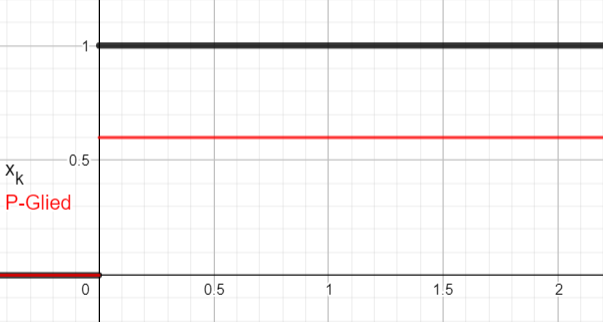
\includegraphics[width=8cm]{Pictures/StepP.png}}
\caption{Sprungantwort eines P-Glieds}
\label{fig:StepP}
\end{center}

\vspace{0.25cm}
\refImgShort{fig:StepPID} zeigt charakteristischen Sprungantwort des \textit{P-Glieds}. Hier wurde der Parameter $k_P$ mit dem Wert 0,6 gewählt, um die Sichtbarkeit in der Abbildung zu erhöhen.
\end{figure}

In einem geschlossenen Regelkreis führt der Einsatz eines \textit{P-Glieds} ohne weitere Regelbausteine zu einer bleibenden Regelabweichung.
Aus den Zusammenhängen $e=w-r$ und $r=e*k_P$\footnote{Für diesen Ansatz werden sämtliche Bausteine nach \textit{E} (\textit{Regelglied}) (siehe \refImg{fig:Contr}) ignoriert. Daraus folgt: $r = m$.} lässt sich die dauerhafte Regelabweichung in Abhängigkeit des Verstärkungsfaktors bestimmen: $e=\frac{w}{1-k_P}$.

Entgegen steht der Vorteil eine schnellen und dauerhaften Reaktion auf eine Regeldifferenz.

\FloatBarrier
\newSec[ControlI]{I-Gield}{3}
Wie sich aus dem Namen des \textit{Integral-Glieds} ableiten lässt, bildet dieser Baustein ein Integral über dem Eingangssignal.
Hierdurch können physikalische Umrechnungen oder Prozesse abgebildet werden. Als Beispiele kann an dieser Stelle der Füllstand eines Tanks oder die Ermittlung einer Geschwindigkeit aus Beschleunigungsdaten genannt werden. \comp{RT1}

\begin{equ}[!ht]
\begin{equation}
y_k = y_{k-1} + k_I * x_k*{\Delta t}
\end{equation}
\caption{Übertragungsfunktion des I-Glieds}
\end{equ}

\begin{figure}[ht!]
\vspace{0.25cm}
\begin{center}
\fbox{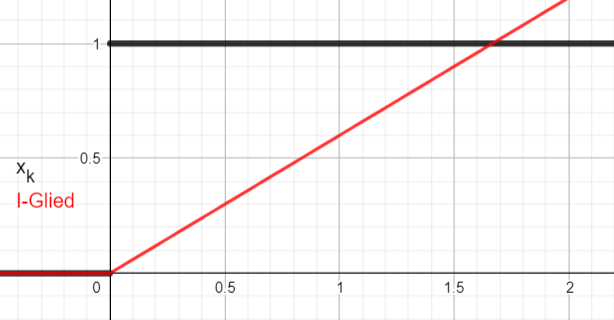
\includegraphics[width=8cm]{Pictures/StepI.png}}
\caption{Sprungantwort eines I-Glieds}
\label{fig:StepI}
\end{center}

\vspace{0.25cm}
\end{figure}

Da das \textit{I-Glied} Regeldifferenzen aufsummiert, läuft die Regeldifferenz im geschlossenen Regelkreis asymptotisch gegen den Wert 0.


\FloatBarrier
\newSec[ControlD]{D-Gield}{3}
In der betrachteten Literatur spielen D-Glieder keine signifikante Rolle. \compB{RT1}{SV1}
Dennoch sollen sie hier als Grundlage für \textit{PID}-Glieder beschrieben werden.

Bei einem \textit{D-Glied} handelt es sich um ein differentielles Glied. Somit lässt sich hiermit die Veränderung des Eingangssignals ermitteln.\comp{ContrD}\missing[Diese Quelle iO?]

Das Ausgangssignal des \textit{D-Glieds} kann durch folgende Formel berechnet werden, welche sich aus der Diskretisierung der Differenztationsfunktion ergibt.

\begin{equ}[!ht]
\begin{equation}
y_k = k_D * \frac{x_k - x_{k-1}}{\Delta t}
\end{equation}
\caption{Übertragungsfunktion des D-Glieds}
\end{equ}

\begin{figure}[ht!]
\vspace{0.25cm}
\begin{center}
\fbox{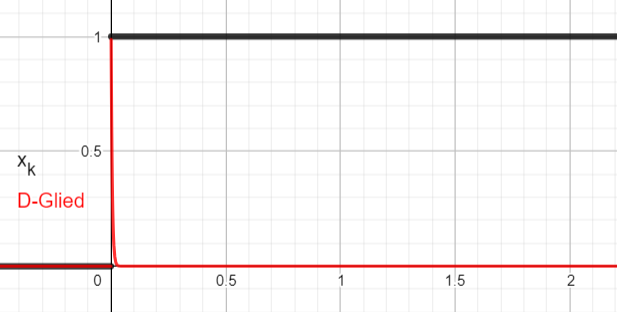
\includegraphics[width=8cm]{Pictures/StepD.png}}
\caption{Sprungantwort eines D-Glieds}
\label{fig:StepD}
\end{center}

\vspace{0.25cm}
\refImgShort{fig:StepD} zeigt die Sprungantwort eines \textit{D-Glieds}. Diese ist ist ein Ausschlag, welcher für den Zeitschritt anhält, in dem sich die ansteigende Flanke des Sprungs befindet.
\end{figure}

Durch den Einfluss eines \textit{D-Glieds} kann auf schnelle Änderungen einer Größe reagiert werden. Die Regeldifferenz der Sprungantwort ist nach dem anfänglichen Ausschlag mit dem Wert 1 (100\%) anzunehmen.


\FloatBarrier
\newSec[ControlPID]{PID-Regler}{3}
Das \textit{PID-Glied} bildet die Vereinigung der vorab genannten Regelbausteine. Als Ausgangssignal wird die Summe über die einzelnen Regelbausteine gebildet:
\begin{equ}[!ht]
\begin{equation}
y_k = y_{k(P)} + y_{k(I)} + y_{k(D)}
\end{equation}
\caption{Übertragungsfunktion des PID-Glieds}
\end{equ}

\begin{figure}[ht!]
\vspace{0.25cm}
\begin{center}
\fbox{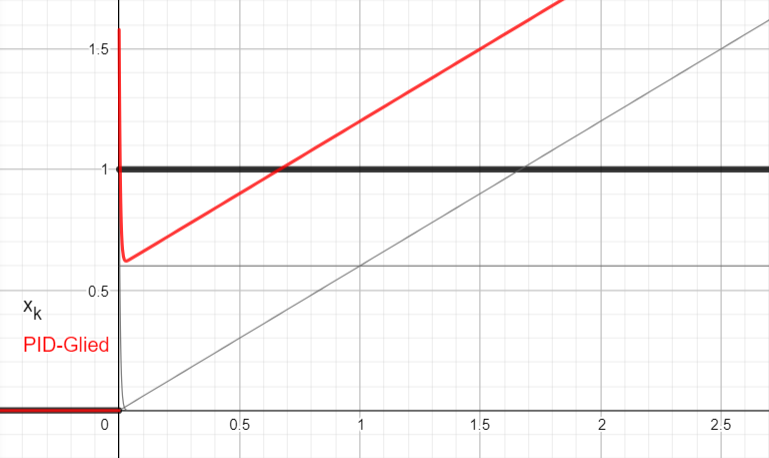
\includegraphics[width=8cm]{Pictures/StepPID.png}}
\caption{Sprungantwort eines PID-Glieds}
\label{fig:StepPID}
\end{center}

\vspace{0.25cm}
\refImgShort{fig:StepPID} zeigt die Sprungantwort eines \textit{PID-Glieds}. Hierbei setzt sich das Signal als Summe des P-, des I- und des D-Glieds zusammen, welche in grau angedeutet sind.
\end{figure}

Das \textit{PID-Glied} vereinigt die Vorteile der Einzelbausteine. Die genannten Nachteile werden durch eines der anderen Regelglieder ausgehebelt.\\
Daher wird das \textit{PID-Glied} als universal-Regelbaustein eingesetzt, wobei geeignete Verstärkungsfaktoren ausgewählt und optimiert werden müssen.


\FloatBarrier
\newSec[ControlPT]{PT-Glied}{3}
Um reale Systeme abzubilden, kann das \textit{PT-Glied} eingesetz werden. Als Beispiele können hier die Temperatur in einem Gas ein eingebrachter Energie oder die Drehzahl eines Motors (massebehaftet) genannt werden.\\
Die Einbindung des \textit{PT-Glieds} erfolgt die Vor- \bzw\ Nachschaltung an Berechnung der idealisierten Größe.


\begin{equ}[!ht]
\begin{equation}
y_k = y_{k-1} + (k_{PT1}*x_k - y_{k-1}) * \frac{\Delta t}{T_1}
\end{equation}
\caption{Übertragungsfunktion des PT-Glieds}
\end{equ}


\begin{figure}[ht!]
\vspace{0.25cm}
\begin{center}
\fbox{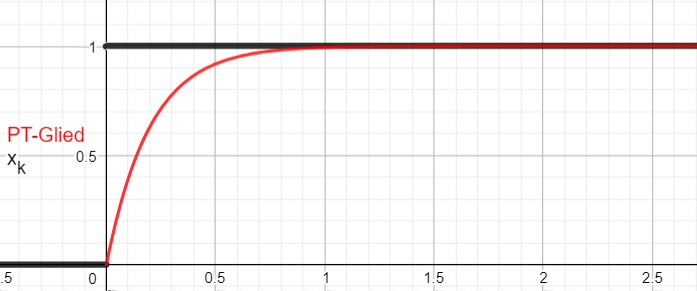
\includegraphics[width=8cm]{Pictures/StepPT.png}}
\caption{Sprungantwort eines PT-Glieds}
\label{fig:StepPT}
\end{center}

\vspace{0.25cm}
\end{figure}




\newSec[ControlPT]{Tt-Glied}{3}
Bei einem \textit{Totzeit-Glied} handelt es sich um Baustein, welcher vorwiegend zur Abbildung realer Systeme genutzt wird. Als Beispiel kann hier die Füllmenge eines Förderbands genannt werden, wobei der Füllstandssensor nach der Befülleinrichtung angeordnet werden muss.\\
Totzeiten erhöhen die Instabilität von Systemen. \missing[Quelle??]

Da dieser Baustein nur zur Vollständigkeit genannt werden soll, wird von einer Vertiefung der Thematik an dieser Stelle abgesehen.


















					% SubSection
\input{211008_MM_T3100_Regelsystem Stabilität.tex}					% SubSection

%\clearpage
%\newSec{Signalverarbeitung}{1}



\missing[irgendwo darauf hinweisen, dass es hier nur online-Verfahren genutzt werden können.]
				% Section
%\input{211008_MM_T3100_Signalverarbeitung Zeitdiskretität.tex}			% SubSection
%\newSec{Messabweichungen}{2}













		% SubSection
%\newSec{Aufarbeitung von Signalen}{2}





\newSec{Median-Filter}{3}







\newSec{Mittelwert-Filter}{3}





\newSec{dauerhafte Nullpunkt-Abweichung}{3}


			% SubSection


\clearpage
\newSec[ControlPos]{Positionsregelung von \Quad[n]}{1}








					% Section
\newSec[ControlPosPose]{Positionsregelung von \Quad[n] mittels Pose}{2}
Die Freiheitsgrade einer Drohne können grundsätzlich separat geregelt werden.
Jedoch ist die Kraft in z-Richtung abhängig von der Ausrichtung (Roll und Pitch) des \Quad[s]. Dies ist aus \refImg{fig:ForcesRolled} ersichtlich. Der \Quad\ wird als Folge einer Veränderung der Roll- und Pitch-Winkel an Höhe verlieren. Der Höhenregler wird diese Veränderung nachführen.
Um ein Nachregeln des \Quad[s] bei einer Orientierungsänderung in der Horizontalen abschwächen zu können, kann der veränderte Schubbedarf aus den gemessenen oder berechneten Roll- und Pitch-Winkeln abgeleitet und zu dem Schubsignal aufsummiert werden.


Es ist zu beachten, dass sie Parallelität des \Quad-Koordinatensystem zum lokalen \bzw\ globalen Koordinatensystem bei einer rotation um die z-Achse verloren geht. Hierzu ist die translative Bewegung entgegengesetzt dieser Rotation zu transformieren. Somit kann die Position bezogen auf das lokale \bzw\ globale Koordinatensystem ermittelt werden. \missing[Quelle? evtl Vorlesung?]


					% SubSection
\newSec[ControlPosAccel]{Erzeugung von Posen aus Beschleunigungsdaten}{2}



					% SubSection



%\clearpage
%\newSec[Topic]{Analyse der verfügbaren ROS-Topics}{1}























\newSec[Msgs]{ROS-Messages}{2}







\newSec[Topics]{ROS-Topics}{2}






\newSec[MavROS]{mavros als Abstraktionsebene}{2}

\textit{mavros} ist eine Bibliothek, welche allgemein für Fluggeräte mit 4 Freiheitsgraden erstellt wurde. Zusätzlich können verschiedene Sensordaten übermittelt werden.























				% Section
%\newSec[TopicTrouble]{Troubleshooting}{2}


\missing[Topics anders benannt, als in Dokumentation (überall steht "/mavros" davor]

\missing[Achtung: der Regler VRA muss so eingestellt sein, dass "manual Flight" verfügbar ist. Andersfalls ist ein Start der Drohne nicht möglich.]


\newSec[TopicTroubleBlacklist]{Clover ist faul}{3}
Um Ressourcen zu sparen werden einige \Topic[s] nicht vom \Pie\ verarbeitet \bzw\ weitergegeben.

\newSec{Lösung}{4}
Unterdrückte \Topic[s] müssen 
\missing[ungetested!]

https://clover.coex.tech/en/mavros.html

Freigegebene \Topic[s] in \texttt{mavros.launch}

\begin{lstlisting}[style=Style_XML, numbers=none, caption={[Freigegebene Topics] Freigegebene \Topic[s] in \texttt{mavros.launch}}]
<rosparam param="plugin_whitelist">
	- altitude
	- command
	- distance_sensor
	- ftp
	- global_position
	- imu
	- local_position
	- manual_control
	# - mocap_pose_estimate
	 - param
	 - px4flow
	 - rc_io
	 - setpoint_attitude
	- setpoint_position
	- setpoint_raw
	- setpoint_velocity
	- sys_status
	- sys_time
	- vision_pose_estimate
	# - vision_speed_estimate
	# - waypoint
</rosparam>
\end{lstlisting}


\newSec[TopicTroubleRCOverMD5]{md5-Sum des Topics OverrideRCIn}{3}
Nach erfolgreicher Kompilierung wird nachfolgender Laufzeitfehler ausgegeben, wenn sich ein \CodeClass{ros::Subscriber} oder ein \CodeClass{ros::Publisher} auf das \rTopic{/mavros/rc/override} anmeldet:\\
\textcolor{red}{[ERROR] [1643616625.226584828]: Client [/mavros] wants topic /mavros/rc/override \\to have datatype/md5sum [mavros\_msgs/OverrideRCIn/73b27a463a40a3eda1f9fbb1fc86d6f3], but our version has [mavros\_msgs/OverrideRCIn/fd1e1c08fa504ec32737c41f45223398]. Dropping connection.}

\newSec{Lösung}{4}
Definition von \\\CodeMeth{struct MD5Sum<::mavros\_msgs::OverrideRCIn\_<ContainerAllocator>>} \\aus 

\begin{lstlisting}[style=Style_Bash, caption=Befehl zum Öffnen des \textit{OverrideRCIn}-Headers]
sudo nano /opt/ros/noetic/include/mavros_msgs/OverrideRCIn.h
\end{lstlisting}

\begin{lstlisting}[style=Style_CPP, numbers=none, caption=Definition des Struct \CodeStruct{MD5Sum} für das Template \textit{OverrideRCIn}]
template<class ContainerAllocator>
struct MD5Sum<::mavros_msgs::OverrideRCIn_<ContainerAllocator>>
{
	static const char* value()
	{
		return "73b27a463a40a3eda1f9fbb1fc86d6f3";
	}

	static const char* value(const ::mavros_msgs::OverrideRCIn_<ContainerAllocator>&)
	{
		return value();
	}
	
	static const uint64_t static_value1 = 0x73b27a463a40a3edULL;
	static const uint64_t static_value2 = 0xa1f9fbb1fc86d6f3ULL;
};
\end{lstlisting}

von dem \Pie\ kopieren und in der Definition des lokalen \ROS\ \textit{\mbox{OverrideRCIn}}-Headers ersetzen.



\newSec[TopicTroubleRCOver]{Topics OverrideRCIn läuft nur mit Topic RCIn}{3}





\newSec{Lösung}{4}









\newSec[TopicTroubleRCOver]{Topics setpoint_altitude/thrust läuft nicht}{3}





\newSec{Lösung}{4}
























			% SubSection

\addtocontents{toc}{\protect\clearpage}			% Seitenumbruch im Inhaltsverzeichnis
\clearpage
\newSec[HW]{Betrachtung der Hardware}{1}



						% Section
\newSec[HWCOEX]{COEX Drohne}{2}

Bei dem für die \DHBW\ neu angeschafften \Quad\ handelt es sich um das Modell \Clover\ des Unternehmens \textit{Copter Express} (\COEX).

Das Modell \Clover\ wurde vom Hersteller zur Ausbildung und Forschung an \Quad[n] entwickelt. Das Modell besitzt einen Rahmen, welche die Rotoren bei Kollisionen schützten soll.




Interner Flight Controller, ROS Kommunikation via Pie 4.




Probleme bei Inbetriebnahme - Beispielprogramm des Herstellers bringt nicht das erwartete Ergebnis.




\newSec[Control]{Control Stack}{3}
Als \textit{Flight Controller} wird das Modell \textit{PX4 Racer} genutzt. Die Firmware, sowie weitere Software zur Interaktion mit der Drohne \Clover\ werden von \textit{Dronecode Foundation} bereitgestellt.

Die Anbindung an \ROS wird durch einen \Pie\ realisiert. Hierbei wird der On-Board Computer als \textit{roscore} genutzt.


\newSec{Funkfernsteuerung}{3}
s-Bus ??





\newSec{Sensorik}{3}

\missing[EIn bisschen Einleitung.]


\begin{itemize}
\item Gyroskop
\item Laser-Abstandsmessung zum Boden
\item GPS
\item Bodenkamera
\end{itemize}










\newSec[Build]{Aufbau des Bausatzes}{3}





\newSec{Aufbau}{4}

\missing[Bilder vom Aufbau]








\newSec[Build]{Inbetriebnahme}{3}


\newSec{Konfiguration des Flight Controllers}{4}



\newSec{Testflug}{4}



\comp{coexExample}
\missing[Verweis auf Example Code]













\newSec[Build]{Mögliche Lösung der Aufgabenstellung}{3}



\newSec[COEXPkg]{COEX-Package}{4}
Für die Interaktion mit der \COEX-Drohne wurden diverse Klassen erstellt, um einzelne Aspekte der Interaktion mit der Drohne umsetzen zu können.

Nach dem Wechsel auf die andere Drohne wurde die Aktualisierung dieses Package nicht weiter verfolgt. Sofern eine Einbindung der \COEX-Drohne in die Ergebnisse dieser \Arbeit\ durchgeführt werden soll, müss dieses Package entsprechend angepasst werden.



\newSec[COEXPkg]{geeignete Topics}{4}

Mit dem \rTopic{blablub} \missing\ kann eine Regelung in der XY-Ebene umgesetzt werden. Die Höhenregelung kann mit set\_attitude/thrust eingeführt werden.
Somit wäre der Versuch für nachfolgende Studierende sehr viel sicherer und so.


\missing\



\newSec[CoexLiteratur]{hilfreiche Literatur}{4}
Nachfolgend sollen Internetseiten genannt werden, welche die Einarbeitung in den Umgang mit der \COEX-Drohne vereinfachen können.

\begin{itemize}
\item https://clover.coex.tech/en/wifi.html

\item https://clover.coex.tech/en/simple\_offboard.html
\item https://docs.px4.io/master/en/ros/mavros\_offboard.html
\item https://docs.px4.io/master/en/flight\_modes/offboard.html

\item https://mavlink.io/en/services/manual\_control.html
\item http://wiki.ros.org/mavros\#mavros.2FPlugins.manual\_control

\item https://mavlink.io/en/messages/common.html\#SET\_POSITION\_TARGET\_LOCAL\_NED
\end{itemize}

Spezifische Verweise sind im Quellcode des \COEX-Package hinterlegt.



\newSec[COEXTrouble]{Troubleshooting}{3}



\missing[Achtung: der Regler VRA muss so eingestellt sein, dass "manual Flight" verfügbar ist. Andersfalls ist ein Start der Drohne nicht möglich.]





\newSec{Platinenfehler}{4}

\missing[Hier anmerken, dass das Problem bisher nicht behoben wurde => Wirkt sich nur auf LED-Streifen aus.]





\newSec{Bus-System des RC Empfängers}{4}
\missing[RC-Empfänger gibt per default i-Bus aus, PX4 erwartet s-Bus.]

\missing[Bild von Oszilloskop]


\texttt{Lösung}\\
\missing[i-Bus und s-Bus werden durch Halten des Knopfens getauscht. Verweis auf Homepage angeben?]





\newSec[TopicTroubleRCOverMD5]{md5-Sum des Topics OverrideRCIn}{4}
Nach erfolgreicher Kompilierung wird nachfolgender Laufzeitfehler ausgegeben, wenn sich ein \CodeClass{ros::Subscriber} oder ein \CodeClass{ros::Publisher} auf das \rTopic{/mavros/rc/override} anmeldet:\\
\textcolor{red}{[ERROR] [1643616625.226584828]: Client [/mavros] wants topic /mavros/rc/override \\to have datatype/md5sum [mavros\_msgs/OverrideRCIn/73b27a463a40a3eda1f9fbb1fc86d6f3], but our version has [mavros\_msgs/OverrideRCIn/fd1e1c08fa504ec32737c41f45223398]. Dropping connection.}

\texttt{Lösung}\\
Definition von \\\CodeMeth{struct MD5Sum<::mavros\_msgs::OverrideRCIn\_<ContainerAllocator>>} \\aus 

\begin{lstlisting}[style=Style_Bash, caption=Befehl zum Öffnen des \textit{OverrideRCIn}-Headers]
sudo nano /opt/ros/noetic/include/mavros_msgs/OverrideRCIn.h
\end{lstlisting}

\begin{lstlisting}[style=Style_CPP, numbers=none, caption=Definition des Struct \CodeStruct{MD5Sum} für das Template \textit{OverrideRCIn}]
template<class ContainerAllocator>
struct MD5Sum<::mavros_msgs::OverrideRCIn_<ContainerAllocator>>
{
	static const char* value()
	{
		return "73b27a463a40a3eda1f9fbb1fc86d6f3";
	}

	static const char* value(const ::mavros_msgs::OverrideRCIn_<ContainerAllocator>&)
	{
		return value();
	}
	
	static const uint64_t static_value1 = 0x73b27a463a40a3edULL;
	static const uint64_t static_value2 = 0xa1f9fbb1fc86d6f3ULL;
};
\end{lstlisting}

von dem \Pie\ kopieren und in der Definition des lokalen \ROS\ \textit{\mbox{OverrideRCIn}}-Headers ersetzen.
Ein Versuch, den \Pie\ einem Update zu unterziehen, ist fehlgeschlagen. Somit ist eine unmittelbare Synchronisation der Nachrichten-Typen aufwändig.


						% SubSection
\newSec[HWParrot]{Parrot Drohne}{2}

Um die Problematik der COEX Drohne zu umgehen, steigt diese \Arbeit\ auf die Drohne um, welche die Idee für diese Studienarbeit ergeben hat.
Hierbei handelt es sich um die Drohne \Ar. Nachfolgend soll die Drohne und die eingebaute Sensorik näher bechrieben werden.



\newSec{Geometrie}{3}


\newSec[parrotGeom]{Anordnung der Rotoren}{4}
\missing

X


\newSec[parrotSize]{Abmessungen}{4}
\missing







\newSec[Control]{Control Stack}{3}

\missing[Bezeichnung auf deutsch?]



\missing[Drohne ist nur Client]

\missing[Nutzung von ardrone\_autonomy-\Pack]




\newSec{Sensorik}{3}


\begin{itemize}
\item Beschleunigungssensorik
\item Magnetometer
\item Ultraschall-Abstandsmessung zum Boden
\item Frontkamera
\item Bodenkamera
\end{itemize}







\newSec[parrotROS]{Interaktion mittels \ROS}{3}



\newSec[parrotAutonomy]{Treiber \pAuto}{4}
Für die Ansteuerung der Drohne \Ar\ existiert eine Treiber, welche die initialisierung und die Kommunukation mit der Drohne anbietet. Als \ROS-seitige Schnittstelle werden verschiedene \Topic[s] und \Service[s] angeboten, welche nachfolgend näher beschrieben werden sollen.


\newSec[parrotTopics]{Topics}{4}




\missing[Bild von rqt-graph]




\newSec[parrotTopicsNav]{\rTopic{NavData}}{5}
Das \rTopic{NavData} fasst alle für die verfügbaren Daten des \Quad[s] in einem Nachricht zusammen. hieraus können geeignete Informationen entnommen werden.


\newSec[parrotTopicsCMD]{\rTopic{cmd\_vel}}{5}
Nur geschwindigkeits-Daten. Keine tatsächliche Übergabe von Neigungswinkeln und so ODER??
\missing\







\newSec[parrotTopicsStream]{Video-Streams}{5}
Die Übertragung der Video-Daten der beiden Kameras soll an dieser Stelle lediglich erwähnt werden.


\newSec[parrotService]{Services}{4}









\newSec[parrotParams]{Parameter}{4}








\newSec[parrotIB]{Inbetriebnahme auf separatem Rechner}{3}


\missing[Batterien halten für knapp 1 Minute oder weniger. Neue wurden bestellt, aber waren erst 3 Wochen vor Abgabe verfügbar. In dieser Zeit wurde maßgeblich an der Ausarbeitung geschrieben.]







\newSec[parrotTrouble]{Troubleshooting}{3}




















					% SubSection



\clearpage
\newSec[Arch]{Entwurf der Software-Architektur}{1}





						% Section




\clearpage
\newSec{Implementierung}{1}



					% Section

\newSec[ImplDomain]{Domain Layer}{2}

Der \textit{Domain Layer} stellt als Teil der \clean\ die Ebene dar, in der allgemein gültige Typen oder Definitionen abgelegt werden können. Nachfolgend werden die Klassen beschrieben, die in diesem Projekt zu dem \textit{Domain Layer} gehören. Sofern nicht anders betitelt, handelt es sich bei den Klassen um Klassen vom Typ \VO.


\newSec{Optional}{4}
Die Klasse \CodeClass{Optional} soll dem Ringbuffer ermöglichen, das Nichtvorhandensein von Einträgen darstellen zu können. Diese Klasse ist als \textit{template} implementiert und enthält neben dem Speicherplatz für die generische Instanz einen bool'schen Wert als Validierung.
Hiermit wird das Arbeit mit \textit{Null-pointern} im Kontext desr Klasse \CodeClass{Ringbuffer} vermieden.
\note{Mit der Verwendung von c++17 ist eine vergleichbare Klasse Teil der Standard-Bibliothek. Die Sprachversion des Projekts ist c++11.}


\newSec{Ringbuffer}{4}
Die Klasse \CodeClass{Ringbuffer} soll einen Ringspeicher abbilden. Hier wird nicht -wie ner Name vermuten lässt- ein Ringspeicher im Sinne einer ringförmig verketteten Liste implementiert. Diese Klasse Kapselt eine \textit{Standard Template Library} (\textit{STL}) vom Typ \CodeClass{std::vector<T>}, wobei bei Überschreiten der maximalen Anzahl an Elementen das vordere Elemente entfernt wird.\\
\note{Die Implementierung der Klasse \CodeClass{std::vector<T>} sieht vor, neue Elemente an das Ende anzuhängen.}


\newSec{TimedValue}{4}
Die Klasse \CodeClass{TimedValue} soll einen mit einem Zeitstemlep versehenen Wert abbilden. Dies wird durch das Erben von den Klassen \textit{Timestamp} und \CodeClass{Value} umgesetzt.


\newSec{Timestamp}{4}
Mit der Klasse \CodeClass{Timestamp} wird ein Zeitstempel eingeführt. Alle \ROS-Nachrichten beinhalten durch die Kapselung der \CodeClass{std\_msgs::Header}-Klasse einen Zeitstempel.


\newSec{Unit}{4}
Mit \CodeClass{Unit} werden Einheiten umgesetzt, um eine korrekte Übergabe von \CodeClass{Value}-Instanzen zur Laufzeit zu gewährleisten.


\newSec{Value}{4}
Die Klasse \CodeClass{Value} bildet einen Wert ab. Sie besteht aus einer \CodeClass{Unit} und einem dazugehöigen Zahlenwert.


\newSec{Vector3D}{4}
Bei der Klasse \CodeClass{Vector3D} handelt es sich um die Abbildung eines Vektors im dreidimensionalen Raum. Zusätzlich wird dem Vektor eine Einheit zugewiesen.
Zudem werden in dieser Klasse grundlegende mathematische Operationen für Vektoren implementiert.


\newSec{SafetyProvider}{4}
Die \CodeClass{SafetyProvider} ist in ihrer Funktionalität abgeschlossen.
Instanzen der \CodeClass{SafetRequirement} werden an einen \textit{SafetyProvider} übergeben. auf Anfrage wird geprüft, ob die übergebenen Instanzen der \CodeClass{SafetRequirement} die erwartungen erfüllen. Ist dies nicht der Fall, wird die \CodeMeth{safetyTriggered} der hinterlegten Instanzen der \CodeClass{SafetReceiver} aufgerufen.


\newSec{SafetReceiver}{4}
Die \textit{full virtual} \CodeClass{SafetReceiver} fordert die Implementierung der \CodeMeth{safetyTriggered}. Hierin definiert die erbende Klasse, wie in Folge einer Verletzung der Sicherheitsanforderungen reagiert werden soll. Allgemein ist hierfür eine Landung des \Quad[s] vorgesehen.


\newSec{SafetRequirement}{4}
Im Sinne des \textit{Open/Close-Principle} wird die \CodeClass{SafetRequirementy} als virtuelle Klasse eingeführt. Hierdurch werden Eigenschaften und Status \bzw\ Flags des \Quad[s] für Sicherheitsfunktionalitäten zugänglich gemacht.


\newSec{SafetyTranslative}{4}
Eine Instanz der \CodeClass{SafetyTranslative} erhält eine Referenz auf eine Instanz der \CodeClass{SafetyProvider}. Ziel dieser Klasse ist es, die Sicherheitsfunktionalität eines anderen \textit{SafetyProvider} als \textit{SafetRequirementy} einbinden zu können.


				% SubSection
\newSec[ImplApp]{Implementierung des Domain Layers - \textit{DroneController} Package}{2}





\newSec{AccelToPos}{4}
\newSec{State}{4}
\newSec{StateHandler}{4}
\newSec{StateTranslator}{4}
		% SubSection
\newSec[ImplAdapter]{Implementierung des Adapter Layers}{2}





\newSec{ActionAdapter}{4}
\newSec{ActionDirection}{4}
\newSec{Transmitable}{4}
				% SubSection
\newSec[ImplPlug]{PlugIn Layer}{2}


				% SubSection
\newSec[ImplPlugParrot]{\textit{parrot} Package}{3}

Die Klassen in diesem \Pack\ entsprechen der vollständigien Implementierung der virtuellen Klassen des \textit{DroneController}-\Pack. Weitere Details sind dem Code zu entnehmen.

Folgende Klassen sind verfügbar:
\begin{itemize}
\item \CodeClass{parrotBattery}
\item \CodeClass{parrotControl}
\item \CodeClass{parrotIMU}
\item \CodeClass{parrotStatus}
\item \CodeClass{parrotTransmitter}
\end{itemize}





					% SubSubSection
\newSec[ImplPlugController]{\textit{Controller} Package}{3}
Die in dieser \Pack\ umfangreiche Vererbungshirarchie wurde umgesetzt, um das parallel hierzu auszuarbeitende \textit{Software Engineering 2}-Projekt ausführlicher umsetzen zu können. Eine schlankeres \Pack\ wäre möglich.\\
Nachfolgend sollen die implementierten Klassen dieses \Pack\ näher erläutert werden:


\newSec{Controllable}{4}
Die virtuelle \CodeClass{Controllable} hält als Attribut eine Ausprägung der Enumeration \textit{ControllerType} und deklariert zudem die Methoden für die Funktionalität, einen Regelparameter \textit{k} verwalten zu können. Diese Funktionalität wird in der \CodeClass{Controller\_Basic} definiert.


\newSec{ControlledOutput}{4}
Mit der \CodeClass{ControlledOutput} werden die Funktionalitäten der Klassen \CodeClass{Controllable} und \CodeClass{Output} vereint.


\newSec[ContrBasic]{Controller\_Basic}{4}
Die \CodeClass{Controller\_Basic} bildet die Grundlage für die in der Implementierung vorhandenen Regelbausteine, ausgenommen der Klasse \CodeClass{ControllerPID}.


\newSec[ContrD]{Controller\_x}{4}
Klassen, welche mit \glqq \CodeClass{Controller\_}\grqq\ beginnen und einen Baustein (vgl. \refCap{Regelerarten}) benennen, implementieren die Funktion des jeweiligen Bausteins.


\newSec{ControllerSystem}{4}
Instanzen der \CodeClass{ControllerSystem} kapseln Instanzen verschiedener Regelbausteine (\CodeClass{Controller\_}). Hierbei können diverse Regelbausteine als Reihenschaltung zusammengefasst werden.\\
\note{In der Implementierung wird diese Klasse nicht aktiv genutzt.}


\newSec{ControllerType}{4}
Bei \textit{ControllerType} handelt es sich um eine Enumeration. Hier können Parameter der Regelbausteine über eine kapselnde Instanz der \CodeClass{ControllerSystem} angepasst werden.\\
\note{Im Projektfortschritt hat sich keine Möglichkeit ergeben, dieses Funktionalität einzusetzen.}


\newSec{Inputable und Input}{4}
Die beiden Klassen ermöglichen einen Daten-Eingang für ein Objekt. Hierbei Besitzt die \CodeClass{Input} einen Pointer auf eine Instanz der \CodeClass{Outputable}.


\newSec{Outputable und Output}{4}
Die beiden Klassen bilden den Output eines Objekts an. Hierbei ist die \CodeMeth{TimedValue getOutput()} eine virtuelle Methode und muss in einer von der \CodeClass{Outputable} erbenden Klasse definiert werden.


\newSec{TimedDifference}{4}
Die \CodeClass{TimedDifference} wurde eingeführt, um ein Datum und einen Zeitstempel zu vereinen. Dies ist für die Berechnung der Regelbausteine notwendig.					% SubSubSection
\newSec[ImplPlugPos]{\textit{PosControl} Package}{3}				% SubSubSection
\newSec[ImplPlugCall]{\textit{calling} \Pack}{3}

Dieses \Pack\ wurde eingeführt, um die Erzeugung neuer \ROS-\Msg[s] zu umgehen. Ferner bildet die Struktur dieser Klassen einen \textit{pull Observer} ab.
Die aufgerufene Methode erhält den Pointer auf die aufrufende Klasse und kann hiermit eine Entscheidung über weitere Aktionen treffen.

\note{Dieses \Pack\ entspricht nicht den Grundsätzen einer \ROS-Programmierung und ist daher nicht weiter zu nutzen. Die Beschreibung dient an dieser Stelle dem Verständnis des Einsatzes dieser Klassen im \textit{coex} \Pack\ und wird darüber hinaus nicht weiter eingesetzt.}



\begin{figure}[ht!]
\vspace{0.25cm}
\begin{center}
\fbox{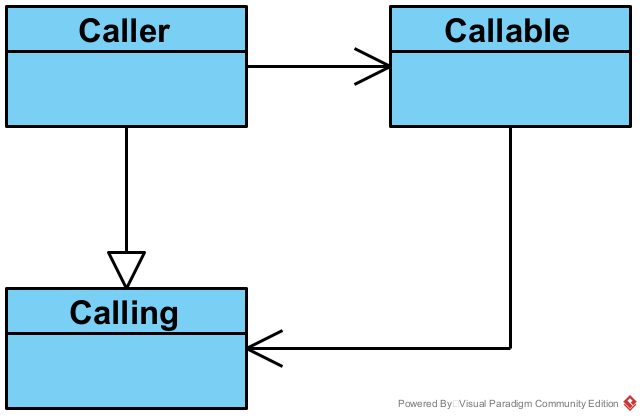
\includegraphics[width=6cm]{Pictures/calling_Pkg.png}}
\caption{Klassendiagramm des \textit{calling} \Pack[s]}
\label{fig:PackCaller}
\end{center}

\vspace{0.25cm}
\end{figure}


					% SubSubSection
\newSec[ArchPlugThread]{\textit{threading} Package}{3}

Das Paket \CodePkg{threading} bietet die Möglichkeit wiederkehrende Aufgaben, abseits von separaten \Node[s], beabeiten zu können. Dieser Zusatz erlaubt ein monolithisches Programm zu entwerfen.


\newSec{Thread}{4}
Diese Klasse bietet die Basis für die Thread-Implementierung, indem die Klasse \CodeClass{std::thread} gekapselt wird. Hier wird mit Aufruf der \CodeMeth{start()}-Methode eine neue Instanz auf den zugehörigen \textit{Pointer} initialisiert. Zusätzlich implementiert die Klasse \CodeClass{Thread} einen Sperr-Mechanismus, um synchrones Schreiben zu vermeiden. \missing[dirty read und so beschreiben?]


\newSec{rosThread}{4}
Die Klasse \CodeClass{rosThread} erweitert die Klasse \CodeClass{Thread} um eine generische Variable \CodeVar{T Payload}, welcher von den erbenden Klassen zum Versand genutzt werden kann. Die Methode \CodeMeth{T runOnce(T Payload)} ist als \textit{full virtual} implementiert, somit wird ein Überschreiben durch erbende Klassen erzwungen. Die Klasse \CodeClass{ros::Rate} ermöglicht eine frequentiell pausierte Abarbeitung des der auszuführenden Methode \CodeMeth{T runOnce()}.

\note{Idealerweise sollte eine Instanz der Klasse \CodeClass{ROS::NodeHandler} ebenfalls in dieser Klasse integriert sein. Tests während der Entwicklung zeigten, dass dies nicht umsetzbar ist. Eine Begründung hierfür konnte nicht gefunden werden.}


\newSec{AutoPublisher}{4}
Wie der Name der Klasse \CodeClass{AutoPublisher} erahnen lässt, wird hier ein \CodeClass{ros::Publisher} implementiert. Mit dem Aufruf der \CodeMeth{runOnce()}-Methode wird wird der in Basisklasse \CodeClass{rosThread} gespeicherte \CodeVar{T Payload} mit der Instanz des \CodeClass{ros::Publisher} versandt.


\newSec{AutoClient}{4}
Die Klasse \CodeClass{AutoClient} kapselt eine Instanz der Klasse \CodeClass{ros::ServiceClient} und bietet somit die Option, Service-Anfragen regelmäßig senden zu können.
Für dieses Projekt ist dies notwendig, da die Anfrage für den \textit{FlightMode} \glqq\texttt{OFFBOARD}\grqq mit einer Frequenz von mindestend $2 Hz$ als \textit{Alive}-Nachricht genutzt wird. Wird die Zeit von $500 ms$ ohne Anfrage überschritten, fällt der \textit{Flight Controller} auf den zuvor verwendeten \textit{FlightMode} zurück.					% SubSubSection
\newSec[ImplPlugCOEX]{\textit{coex} \Pack}{3}

Dieses Kapitel beschreibt die Klassen, welche zur Interaktion mit der zuerst eingesetzten Hardware genutzt wurden.


\note{Die Implementierung dieses \Pack[s] wurde vor der konzeptionellen Änderung des \textit{Application-Layers} umgesetzt.
Die Beschreibung der Klassen dieses Paketes dient der Einarbeitung nachfolgender Studienarbeiten. Auf Grund der Änderungen im Code kann dieses \Pack\ nicht Kompiliert werden.}

\missing[Hier evtl den Abhängigkeitsgraph für coex zur Veranschaulichung?]




\newSec{coexBattery}{4}
Wie der Klassenname vermuten lässt überwacht diese Klasse die Batteriestand des \Quad[s].
\\Diese Klasse entspricht der Klasse \CodeClass{parrotBattery} der \Ar.


\newSec{coexControl}{4}
Die Klasse \CodeClass{coexControl} ist als Fassade eingesetzt und bietet Anwendenden zugriff auf diverse Funktionen der gekapselten Klassen.
\\Diese Klasse entspricht der Klasse \CodeClass{parrotControl} der \Ar.


\newSec{coexMC}{4}
Die Abkürzung \textit{MC} im Klassennamen steht für \textit{Manual Control} und deutet hiermit sowohl das genutzte \Topic\ als auch den zugrundeliegenden Nachrichtentyp an. Laut Entwickler-Literatur (siehe \refCap{CoexLiteratur}) werden Steuerungsdaten der vier Freiheitsgrade an den \Quad\ gesendet. 

Diese Klasse erbt von der Klasse \CodeClass{coexTransmitable}
\\Diese Klasse entspricht der Klasse \CodeClass{parrotTransmitter} der \Ar.


\newSec{coexOrientation}{4}
Es war geplant, die Pose des \Quad[s] in dieser Klasse berechnen zu lassen. Im weiteren Projektverlauf hat sich ergeben, hierfür eine separate Klasse zu erstellen.
\\Diese Klasse entspricht der Klasse \CodeClass{parrotIMU} der \Ar.


\newSec{coexRC}{4}
\CodeClass{coexRC} ist als Fassade für die beiden nachfolgenden implementiert.


\newSec[coexRCR]{coexRC\_Receiver}{4}
Die Klasse \CodeClass{coexRC\_Receiver} liest vom \rTopic{/mavros/rc/in} und somit die Eingaben der Funkfernsteuerung. Eine nähere Erläuterung, welche Daten übermittelt werden, findet sich als Kommentar im Code.


\newSec[coexRCT]{coexRC\_Transmitter}{4}
Als \textit{RC-Transmitter} wird die Klasse bezeichnet, welche Nachrichten an das \rTopic{/mavros/rc/override} veröffentlicht (vgl. \refCap{COEXPkgTopic}).

Diese Klasse erbt von der Klasse \CodeClass{coexTransmitable}


\newSec{coexState}{4}
Die Klasse \CodeClass{coexState} übernimmt die Interaktion mit dem Zustandsautomaten, welcher im \textit{Flight Controller} des \Quad[s] realisiert ist.
Anfragen zur Änderung eies Zustand beziehen sich maßgeblich auf den Start und die Landung eines Flugs.
\\Diese Klasse entspricht der Klasse \CodeClass{parrotStatus} der \Ar.


\newSec{coexTransmitable}{4}
Diese Klasse erbt von der Klasse \CodeClass{Transmitable}. Hierin wird die Steuerung innerhalb dieses \Pack[s] als eine normierte \textit{Manual Control}-Nachricht mit dem Wertebereich [-1, 1] definiert.


\newSec{Joystick}{4}
Hier wird ein Hilfskonstrukt für die Transformation von Daten der Funkfernsteuerung eingeführt. Die Klasse implementiert vier Instanzen der Klasse \CodeClass{JoystickAxis}.


\newSec{JoystickAxis}{4}
Hier werden die Rohdaten der Kanäle der Funkfernsteuerung in normierte Daten zu überführt. Zudem können normierte Werte in den Wertebereich der Funkfernsteuerung transformiert werden.

					% SubSubSection




\clearpage
\newSec{Ergebnis}{1}

Um ein Ergebnis bewerten zu können, wird nachfolgend einer Auswahl aussagekräftiger Daten eines Fluges gezeigt. Hierbei wurden zwei Starts in dem Datendatz durchgeführt. Zur besseren Interpretation wurden Daten entfernt, welche entsprechend der Implementierung irrelevant sind.

Ein Mitschnitt, welcher mittels \textit{rosbag} entstand, ist verfügbar. Die genannten Daten wurden mittels geeigneter Software (\texttt{rosrun BagPlotter parrot} und \texttt{rosbag play <File>.bag}) in menschenlesbare \textit{.txt} Dateien überführt. Diese Daten wurden anschließend zur Ermittlung der von der Implementierung geschätzten Pose genutzt. Dieser Vorgang wurde aus Sicherheitsgründen in einer Simulation (\textit{PosControl/Simulant.cpp}) durchgeführt.




Im Zuge dieses Projekts wurden diverse Sicherheitsfunktionen zum \Quad\ hinzugefügt. Da sich diese \Arbeit\ aus interne Sensoren beschränkt, werden diese als Basis der Sicherheitsfunktionen eingesetzt.
Aus den übertragenen Daten kann ein Timeout\footnote{Der \textit{Timeout} wird in diesem Projekt mit dem Eingang einer neuen Nachricht ermittelt. Geeigneter wäre das Starten eines Timers beim Eingang einer Nachricht. Verstreicht die Zeit des Timers soll das Landemanöver initialisiert werden.}, sowie ein Zusammenstoß mit einem Objekt ermittelt werden. Als weitere Funktionalität wird ein Absturz auf Grund einer zu geringen Akku-Ladung verhindert. Jedes Sicherheitsfunktion löst das Landemanäver der \Ar\ aus.
















						% Section
\newSec[Flight]{Analyse realer Flugdaten}{2}

\newSec[FlightData]{Datenbasis}{3}
Dieses Kapitel zeigt die verschiedenen Daten des Flugs, um diese in der nachfolgenden Analyse einordnen zu können.

Der gezeigte Datensatz enthält zwei Flüge, welche naheinander aufgenommen wurden. Aus diesen Daten wurden irrelevante Einträge zwischen den Flügen entfernt. Durch diesen Eingriff wurde der berechnete Verlauf des zweiten Fluges nicht beeinflusst, da die Status des \Quad\ zu geeigneten Zeitpunkten zurückgesetzt werden.

Der vom Zustandsautomaten der \Ar\ einnehmbare ZustandIDs sind im \CodePkg{ardrone\_autonomy} wie folgt definiert:
\begin{table}[!ht]
\begin{tabular}{ll}
StatusID & Status-Text    \\ \hline
0        & Unknown        \\
1        & Init           \\
2        & Landed         \\
3        & Flying         \\
4        & Hovering       \\
5        & Test           \\
6        & Taking off     \\
7        & Goto Fix Point \\
8        & Landing        \\
9        & Looping       
\end{tabular}
\end{table}
\FloatBarrier
Aus den Flugversuchen zeigte sich, dass StatusID 6 (\textit{Taking off}) nicht gesendet wird. Stattdessen wird StatusID 7 (\textit{Goto Fix Point}) unmittelbar nach der \textit{Takeoff}-Message eingenommen. StatusID 8 (\textit{Landing}) wird durch StatusID 9 (\textit{Looping}) abgebildet. 


\begin{figure}[ht!]
\vspace{0.25cm}
\begin{center}
\fbox{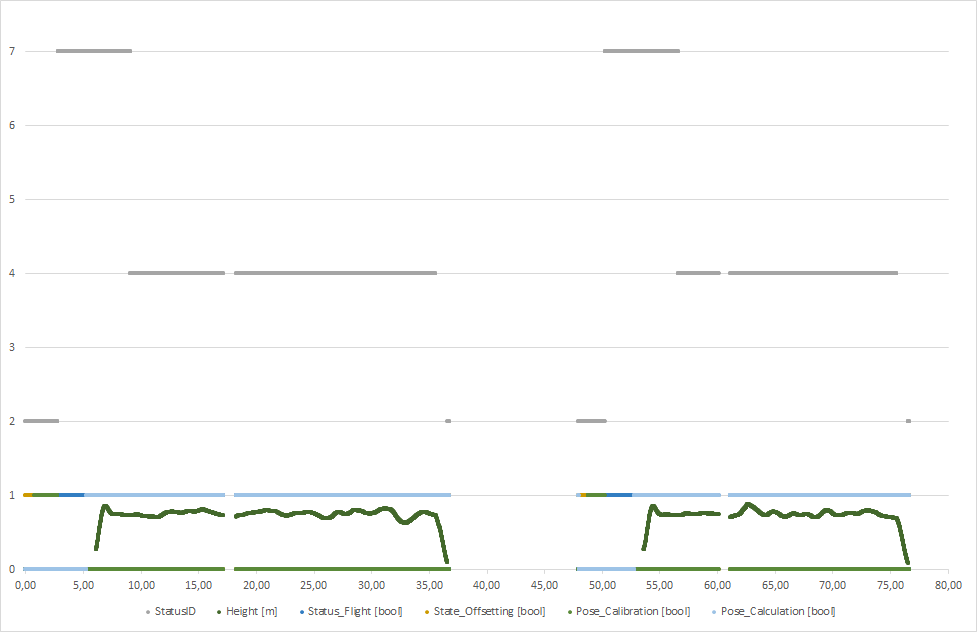
\includegraphics[width=15cm]{Pictures/TestFlight Status Flags Height.png}}
\caption{Testflug: StatusID}
\label{fig:FlightStatus}
\end{center}

\vspace{0.25cm}
Um die Aussagekraft der Graphik zu gewährleisten wurde die Ordinatenachse lediglich bis zum Wert 7 abgebildet. Hierdurch wird die StatusID der Landephase ausgespart.
\end{figure}

Aus den Daten kann eine \textit{ground truth} für die Position der z-Achse entnommen werden. Diese Daten stammen von dem auf den Untergrund gerichteten Ultraschall-Sensor.\\
Eine Genaue Abschätzung der Korrektheit dieser Daten lässt sich nicht aus Vergleichsdaten belegen. Die Genauigkeit des Untraschall-Sensors kann jedoch als höher angenommen werden als die der berechneten Pose.


\FloatBarrier
\newSec[FlightProcess]{Verlauf des Fluges}{3}

\missing[Hier Abb 18 detailliert geschreiben. Besonders auf Flags eingehen.]







\newSec[FlightAnalysisLeak]{Lecks der Datenübertragung}{3}
Aus den Daten, aufgetragen in \refImg{fig:FlightStatus}, und weiteren Testflugen zeigt sich, dass die Verbindung zwischen dem Host-PC und dem \Quad\ anfällig für Verbindungsunterbrechnungen ist. Während diesen Unterbrechnungen werden für einen Zeitraum von etwa einer Sekunde keine Nachrichten übermittelt. 

Die entwickelte Software sieht für diese Fälle keine Interpolation der Daten vor. Hieraus entstehen Sprünge in den berechneten Daten. Hier können als Beispiel \refImg{fig:FlightPoseVel} und \refImg{} jeweils für die Zeitbereiche um 17 Sekunden und 61 Sekunden herangezogen werden.
\missing[Bild der berechneten Pose referenzieren.]







					% SubSection
\newSec[Signals]{Signalverarbeitung}{2}


\newSec[SignalsOffsetCalc]{Ermittlung der dauerhaften Nullpunkt-Abweichung}{3}
In \refImg{fig:SzeneOffset} wird eine Abweichung der Beschleunigungswerte vom Nullpunkt deutlich. Die eingesetzte Software wirkt dem in der \CodeClass{StateBuilder} entgegen, indem über eine definierte Anzahl an Eingangswerten der \CodeClass{IMUState} ein Mittelwert gebildet wird. Um an dieser Stelle aussagekräftigere Ergebnisse zu erhalten, wird zudem die Varianz über den zwischengespeicherten Datensatz gebildet. Der Mittelwert mit der geringste Varianz aus einer definierten Anzahl an Stichproben wird als Nullpunkt-Abweichung angenommen. Hierbei ist zu beachten, dass die Attribute der \CodeClass{IMUState} separat betrachtet werden.

\begin{figure}[ht!]
\vspace{0.25cm}
\begin{center}
\fbox{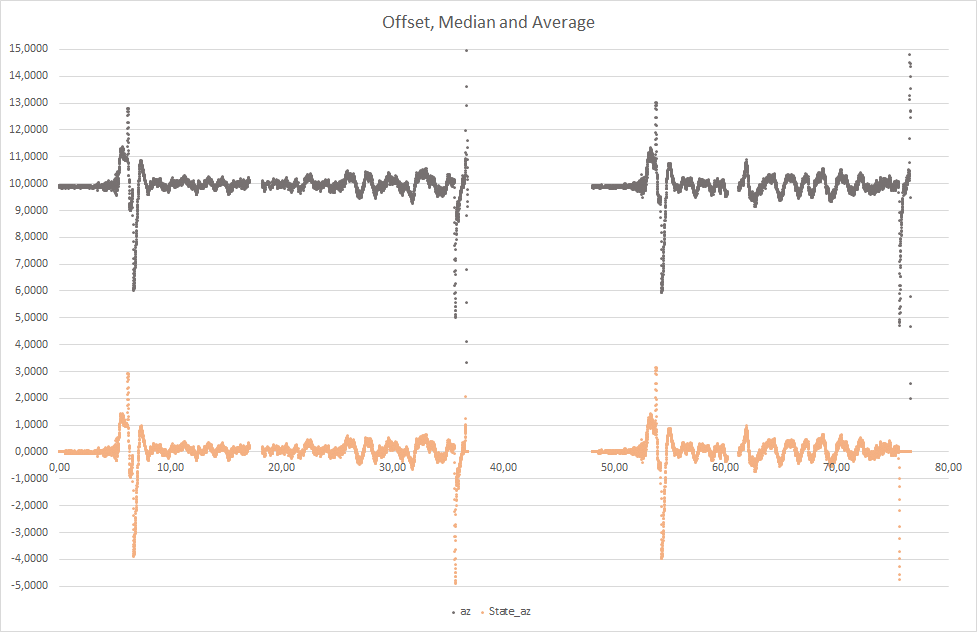
\includegraphics[width=12cm]{Pictures/TestFlight State_az Med1 Avg1 Off50 Calib1.png}}
\caption{Testflug Signalverarbeitung: Aufarbeitung $a_z$}
\label{fig:FlightStatusaz}
\end{center}

\vspace{0.25cm}
\refImgShort{fig:FlightStatusaz} zeigt die erfolgreiche Ermittlung der dauerhaften Nullpunkt-Abweichung für die Beschleunigungswerte entlang der z-Achse.\\
Es zeigt sich, dass die Nullpunkt-Abweichung aus den Eingangsdaten der \Quad-IMU berechnet und als Grundlage für eine weitere Aufarbeitung der Daten eingesetzt werden kann.
\end{figure}


\newSec[SignalsSmooth]{Glättung der Eingangsdaten}{3}
Als Parameter werden für die Berechnung der dauerhaften Nullpunkt-Abweichung (siehe \refCap{SignalsOffsetCalc}) jeweils ein Median-Fenster und ein Mittelwert-Fenster der Größe 1 angesetzt, somit findet keine Veränderung durch diese Filter statt. Es zeigte sich in den Auswertungen, dass ein Median-Fenster bis zur Größe von 15 Werten keinen signifikanten Einfluss auf die berechnete Pose besitzt. Jedoch wirkt sich eine Vergrößerung des Mittelwert-Fensters negativ auf die berechnete Pose aus. Die Abweichung von erwarteten Werten nimmt deutlich zu.


\newSec[SignalsOffsetCalib]{Kalibrierung der Posenberechnung}{3}
Aus Simulationen mit der in \refCap{Implementierung} beschrieben Software zeigte sich, dass eine einfach Abschätzung der Nullpunkt-Abweichung unach \refCap{SignalsOffsetCalc} nicht vollständig ausreicht. Der Einfluss bereits kleiner Nullpunkt-Abweichung wurde in \refCap{ControlPosAccelOffset} erläutert. Aus Erkenntnissen, aufgezeigt in \refImg{fig:SzeneOffset}, lässt sich nachfolgender mathimatische Zusammenhang ableiten:

\begin{equ}[!ht]
\begin{equation}
\Delta P_{Direction}=\frac{\Delta a_{Direction}}{2}*\Delta t^2
\end{equation}
\label{equ:OffsetCalib}
\caption{mathematische Grundlage der \textit{PoseBuildable}-Kalibrierung}
\end{equ}

Entsprechend dieser Formel berechnet die \CodeClass{PoseBuilder} eine nach der Aufarbeitung durch die \CodeClass{StateBuilder} verbleibende Nullpunkt-Abweichung der Beschleunigungswerte. Diese werden zur Berechung der Pose von den Eingangdaten subtrahiert.

In \refImg{fig:FlightPoseVel} kann gezeigt werden, dass sich eine zusätzliche Kalibrierung der Beschleungungsdaten positiv auf die Berechnung der Pose\footnote{In der genannten Abbildung werden die berechneten Geschwindigkeiten aufgetragen.} auswirken kann. Die durch die \CodeClass{PoseBuildable} berechnete Geschwindigkeit entlang der z-Achse entspricht für den zweiten Flug etwa der aus dem gemessenen Höhenverlauf abgeleiteten Geschwindigkeit.

\begin{figure}[ht!]
\vspace{0.25cm}
\begin{center}
\fbox{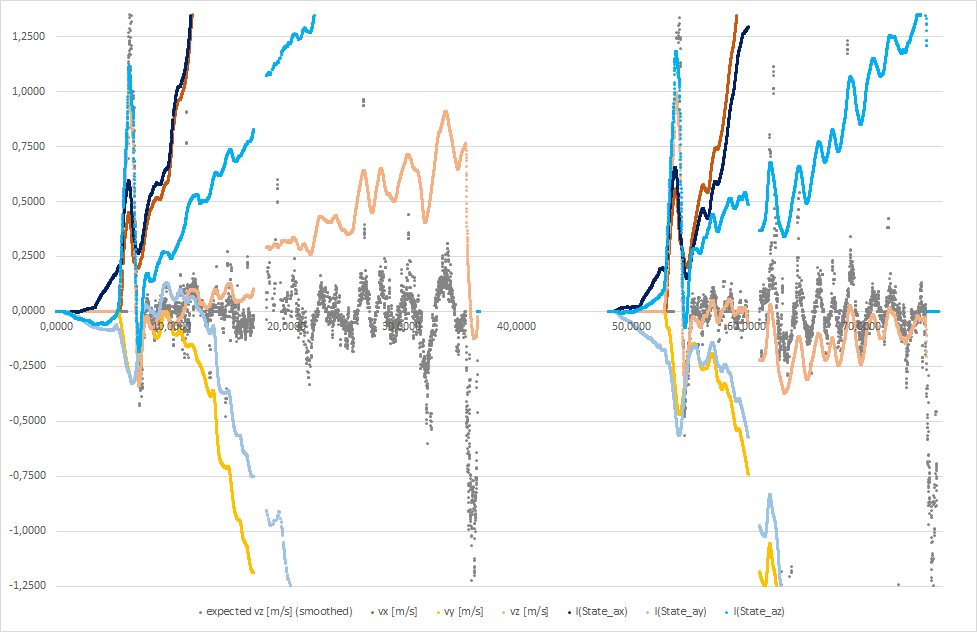
\includegraphics[width=15cm]{Pictures/TestFlight Velocity Med1 Avg1 Off50 Calib1.png}}
\caption{Testflug Signalverarbeitung: Kalibrierung}
\label{fig:FlightPoseVel}
\end{center}

\vspace{0.25cm}
An der aufgetragenen Geschwindigkeit \textit{vz} lässt sich deutlich erkennen, welchen Einfluss die Kalibrierung der \CodeClass{PoseBuildable} hat. Die berechnete Geschwindigkeit (beige) weicht nur mäßig von der erwarteten Geschwindigkeit (grau) ab.\\
\note{Da die \textit{IMU}-Nachrichten in einer Folgen mit kurzen Zeitschritten eintreffen, wurde die erwartete Geschwindigkeit als gleitender Mittelwert über 10 Werte geglättet.}
\end{figure}



















				% SubSection


\clearpage
\newSec{Erweiterungen}{2}

Dieses Kapitel soll beschreiben, welche weiteren Sensoren eingesetzt werden können, um die Genauigkeit berechneten der Pose zu erhöhen.\\
Da es sich bei den möglichen Erweiterungen um eine Fülle von Varianten handelt, sollen diese jeweils nur knapp beschrieben oder lediglich namentlich genannt werden.



\newSec{Weitere Ansätze der Signalverarbeitung / Pose-Berechnung}{3}





\newSec{Interne Sensoren}{3}

\newSec{Höherwertige Initialsensoren}{4}


\newSec{Magnetometer}{4}



\newSec{Externe Sensoren}{3}


\newSec{Bodenkamera}{4}


\newSec{Frontkamera}{4}



\newSec{GPS}{3}

globale Ausrichtung




\newSec{Externe Sensoren und Mapping}{3}




\newSec{Dedektion der Umgebung}{2}

\missing[Auswertung von Objekten und Speicherung der zugehörigen Metadaten]



\newSec{Vorwärts-Berechnung}{3}







\newSec{Rückwärts-Berechnung bei Ringschluss}{3}

\missing[Position und Genauigkeit der vorherig ermittelten Objekte berechnen, wenn ein bekanntes Objekt erneut gesichtet wurde.]

Aufzeichnung des Weges erforderlich



\newSec{Sensoriken}{2}

\newSec{Abstandssensoren}{3}



\newSec{Punktuelle Abstandsmessung}{4}



\newSec{Linienförmige Abstandsmessung}{4}


\newSec{3D Abstandsmessung}{4}




























					% Section




\clearpage
\newSec[Fazit]{Fazit und Ausblick}{1}




							% Section

\clearpage
\PagestyleStdSuf
\clearpage
\addcontentsline{toc}{section}{Literaturverzeichnis}
\newcounter{IndexLiteratur}
\newcommand{\NewBibItem}[2]{\stepcounter{IndexLiteratur} \bibitem[\theIndexLiteratur]{#1} #2,\newline}

% Layout Commands
\newcommand{\Published}[1]{veröffentlicht #1}
\newcommand{\Modified}[1]{verändert #1}
\newcommand{\Requested}[1]{abgefragt #1}
\newcommand{\Online}[1]{online,  #1\newline}
\newcommand{\Version}[1]{#1. Auflage}
\newcommand{\ISBN}[1]{ISBN #1}
\newcommand{\Article}[1]{Artikel \textit{#1}}
\newcommand{\Chapter}[1]{Kapitel \textit{#1}}
\newcommand{\Pages}[1]{Seite #1}
\newcommand{\NA}{-unbekannt-}



\begin{thebibliography}{\theIndexLiteratur}

% Paper
\NewBibItem{Paper1}{Pozo D., Romero L., Rosales J., Quadcopter stabilization by using PID controllers}
\Published{2014}

\NewBibItem{Paper2}{Fresk E., Nikolakopoulos G., Full Quaternion Based Attitude Control for a Quadrotor}
\Published{19.07.2013}


% Bücher




% Einleitung
\NewBibItem{Einl1}{Mey R., Reinhard Mey Textsammlung 14.Auflage}
\Online{https://www.reinhard-mey.de/texte-fuer-alle/}
\Published{13.12.2017}, \Requested{08.02.2022}







% Problemstellung
\NewBibItem{Ballon}{ellwangen2010, Ballon steuern?}
\Online{https://www.ballonfahrten.com/ballon-steuern/}
\Published{20.02.2010}, \Requested{07.11.2021}



% ROS
\NewBibItem{ros1}{ROS - Robot Operating System}
\Online{https://www.ros.org}
\Published{\NA}, \Requested{28.11.2021}

\NewBibItem{rosVersion}{ROS Indigo Igloo}
\Online{http://wiki.ros.org/indigo}
\Published{\NA}, \Modified{08.01.2018}, \Requested{16.03.2022}







%Hardware





%Software





%COEX
\NewBibItem{coexExample}{MAVROS Offboard control example}
\Online{https://docs.px4.io/master/en/ros/mavros\_offboard.html}
\Published{\NA}, \Modified{02.02.2021}, \Requested{16.03.2022}






%Parrot
\NewBibItem{parotSDK}{AR.Drone Developer Guide}
\Chapter{AR.Drone 2.0 Overview}, \Pages{5 ff.}
\Online{https://jpchanson.github.io/ARdrone/ParrotDevGuide.pdf}
\Published{21.05.2012}, \Requested{17.03.2022}










%Language
\NewBibItem{cpp1}{Saks D., Better even at the lowest levels}
\Online{https://www.embedded.com/better-even-at-the-lowest-levels/}
\Published{01.11.2008}, \Modified{05.12.2020}, \Requested{28.07.2021}

\NewBibItem{c1}{Application Note Object-Oriented Programming in C}
\Online{https://www.state-machine.com/doc/AN\_OOP\_in\_C.pdf}
\Published{06.11.2020}, \Requested{28.07.2021}

\NewBibItem{DyString}{Kirk N., How do strings allocate memory in c++?}
\Online{https://stackoverflow.com/questions/18312658/how-do-strings-allocate-memory-in-c}
\Published{19.08.2013}, \Requested{17.08.2021}

\NewBibItem{Dy1}{Bansal A., Containers in C++ STL (Standard Template Library)}
\Online{https://www.geeksforgeeks.org/containers-cpp-stl/}
\Published{05.03.2018}, \Modified{12.07.2020}, \Requested{17.08.2021}

\NewBibItem{DefASA}{Automatic Storage Duration}
\Online{https://www.oreilly.com/library/view/c-primer-plus/9780132781145/ch09lev2sec2.html}
\Published{\NA}, \Requested{17.08.2021}

\NewBibItem{DefDSA}{Noar J., Orda A., Petruschka Y., Dynamic storage allocation with known durations}
\Online{https://www.sciencedirect.com/science/article/pii/S0166218X99001754}
\Published{30.03.2000}, \Requested{17.08.2021}




%Varianten




\end{thebibliography}

\Anmerkung{Wird hier ein Veröffentlichungsdatum als \grqq -unbekannt-\grqq\ markiert, so konnte diese Angabe weder auf der entsprechenden Webseite, noch in deren Quelltext ausfindig gemacht werden.}

\clearpage





\appendix
\renewcommand{\thesection}{\Alph{section}}
\renewcommand{\thefigure}{\thesection.\Roman{figure}}
\setcounter{figure}{0} 
\cleardoublepage
\appendixpage
\clearpage
\PagestyleStdAppendix








\end{document}